\documentclass[a4paper]{article}
\usepackage{amsfonts}
\usepackage{amsmath}
\usepackage{amssymb}
\usepackage{graphicx}
\usepackage{extarrows}

\newcommand{\limit}{\lim\limits}

\begin{document}

\noindent \large Auteur: Seda Jusjajeva\\
\noindent \large Studierichting: Informatica\\
\noindent \large Oefeningenreeks 3H nr. 8.7 \\

\medskip

\normalsize

$r = 2\cos6\theta$ \\

$\operatorname{dom}f = \mathbb{R}$ \\

Periode: $\dfrac{\pi}{3}$ \\

We beperken ons tot het interval $\left[0,\dfrac{\pi}{3}\right]$. \\

Nulpunten: $2\cos6\theta = 0 \Leftrightarrow 6\theta = \dfrac{\pi}{2} + k\pi \Leftrightarrow \theta = \dfrac{\pi}{12} + k\dfrac{\pi}{6} \quad (k \in \mathbb{Z})$ \\

Nulpunten in het interval: $\left\{\dfrac{\pi}{12},\dfrac{\pi}{4}\right\}$ \\

Afgeleide: \\

$r' = \dfrac{d}{dx}(2\cos6\theta) = -2\sin6\theta \cdot \dfrac{d}{dx}(6\theta) = -12\sin6\theta$ \\

Nulpunten: $-12\sin6\theta = 0 \Leftrightarrow 6\theta = k\pi \Leftrightarrow \theta = k\dfrac{\pi}{6} \quad (k \in \mathbb{Z})$ \\

Nulpunten in het interval: $\left\{0,\dfrac{\pi}{6},\dfrac{\pi}{3}\right\}$ \\

Tekenonderzoek: \\

$\begin{array}{r|ccccccccc}	
  \theta & 0 &          &\dfrac{\pi}{12} &          & \dfrac{\pi}{6} &          & \dfrac{\pi}{4} &          & \dfrac{\pi}{3}\\ 
  \hline
  r      & + & +        & 0              & -        & -              & -        & 0              & +        & +\\
  r'     & 0 & -        & -              & -        & 0              & +        & +              & +        & 0\\ 
  \hline
  r      & M & \nearrow & \nearrow       & \nearrow & m              & \searrow & \searrow       & \searrow & M\\
         & 2 &          &                &          & -2             &          &                &          & 2\\
\end{array}$ \\

Grafiek: zie volgende pagina \\

\begin{figure}[h]
\centering
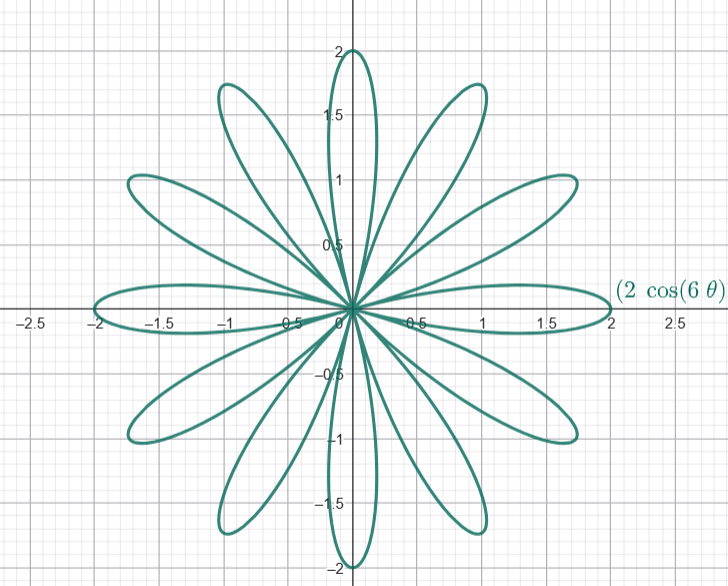
\includegraphics[width=\linewidth]{3H-8.7-seda.jusjajeva.INF.png}
\end{figure}


\begin{thebibliography}{999}
%\bibitem{a} Referentie
\end{thebibliography}
\end{document}